\documentclass{standalone}
\usepackage{tikz}
\usetikzlibrary{patterns}
\begin{document}
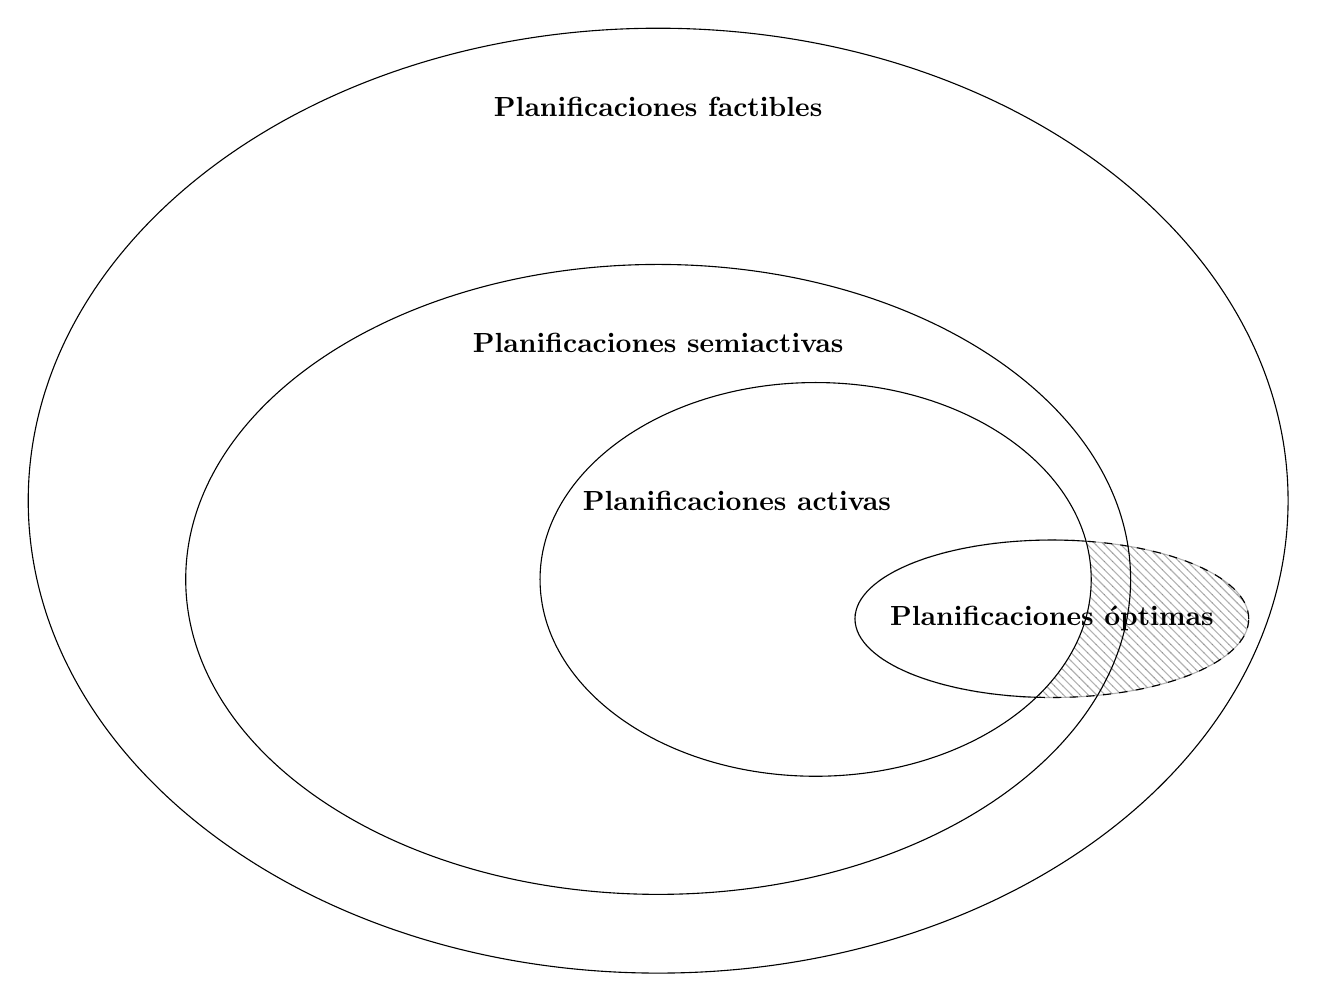
\begin{tikzpicture}
    \draw[fill,pattern=north west lines,opacity=.3](13,4.5) ellipse (2.5 and 1);
    \draw[dashed] (13,4.5) ellipse (2.5 and 1);

    \node [at={(8,11)}] {\textbf{Planificaciones factibles}};
    \draw (8,6) ellipse[x radius = 8,y radius = 6];
    
    \draw (8,5) ellipse[x radius = 6, y radius = 4];
    \node [at={(8,8)}] {\textbf{Planificaciones semiactivas}};
   

    % Intersection
    \begin{scope}
        % factibles
        %\clip (8,6) ellipse (8 and 6);
        % semiactivas
        %\clip (8,5) ellipse (6 and 4);
        % optimas
        \clip (13,4.5) ellipse(2.51 and 1.01);
        % activas
        \clip (10,5) ellipse (3.5 and 2.5);
        
        %\clip (0,0) rectangle (16,12);
        %\fill[black](13,4.5) ellipse(2.5 and 1);
        \fill[white](16,6) rectangle(10,2);
        \draw (13,4.5) ellipse (2.5 and 1);
    \end{scope}
    \node [at = {(13,4.5)}] {\textbf{Planificaciones \'optimas}};
    \node [at={(9,6)}] {\textbf{Planificaciones activas}};
    \draw (10,5) ellipse[x radius = 3.5, y radius = 2.5];
\end{tikzpicture}

\end{document}
